% Appendix C
\g
\chapter{Παράρτημα Κεφαλαίου 3} % Main appendix title

\label{AppendixC} % For referencing this appendix elsewhere, use \ref{AppendixA}

\section{Γνωστές αρχιτεκτονικές νευρωνικών δικτύων για την αρχικοποίηση κόστους}
\label{appendix:common_techniques}

Στις εικόνες \ref{fig:zagoruyko}, \ref{fig:jzbontar}, \ref{fig:luo}, \ref{fig:gydaris} και \ref{fig:kendall} φαίνονται σχηματικά οι γνωστότερες αρχιτεκτονικές που έχουν προταθεί για την αρχικοποίηση του πίνακα κόστους.

\begin{figure}
	\centering
	\begin{subfigure}{0.49\textwidth}
		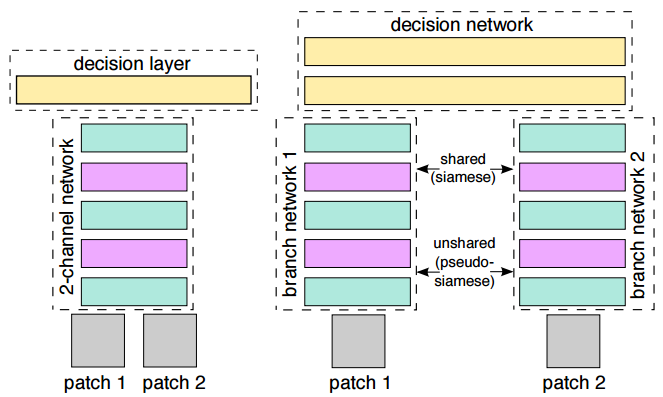
\includegraphics[width=\textwidth]{Zagoruyko1.png}
	\end{subfigure}
	\begin{subfigure}{0.49\textwidth}
		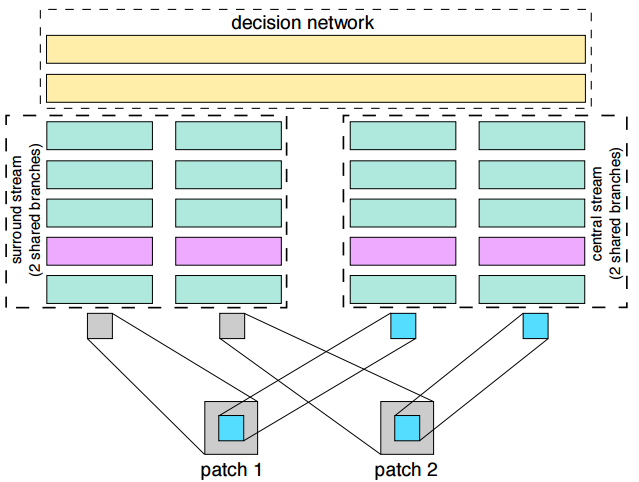
\includegraphics[width=\textwidth]{Zagoruyko2.png}
	\end{subfigure}
	\caption{Αρχιτεκτονικές νευρωνικών δικτύων για την σύγκριση περιοχών εικόνας, όπως προτάθηκαν από τους \e Zagoruyko, Komodakis. \g \citep{zagoruyko2015learning}}
	\label{fig:zagoruyko}
	
	\begin{subfigure}{0.49\textwidth}
		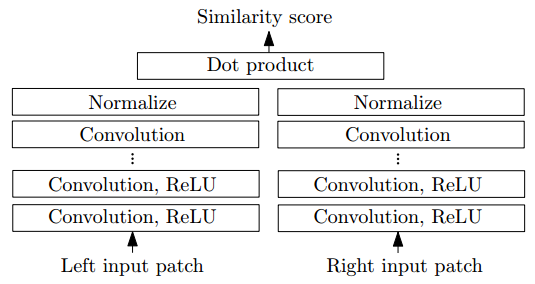
\includegraphics[width=\textwidth]{jzbontar_fast.png}
	\end{subfigure}
	\begin{subfigure}{0.49\textwidth}
		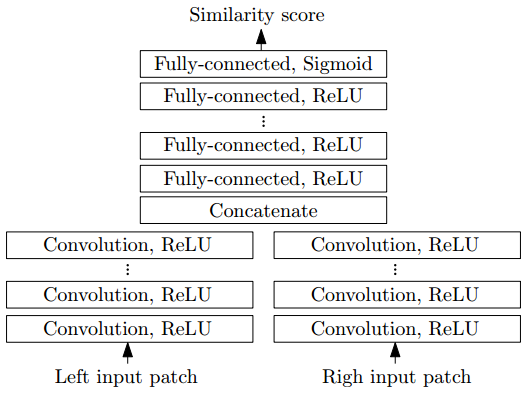
\includegraphics[width=\textwidth]{jzbontar_acc.png}
	\end{subfigure}
	\caption{Αρχιτεκτονικές νευρωνικών δικτύων για την σύγκριση περιοχών εικόνας, όπως προτάθηκαν από τους \e Zbontar, Lecun. \g \citep{zbontar2016stereo}}
	\label{fig:jzbontar}
	
	\begin{subfigure}{0.8\textwidth}
		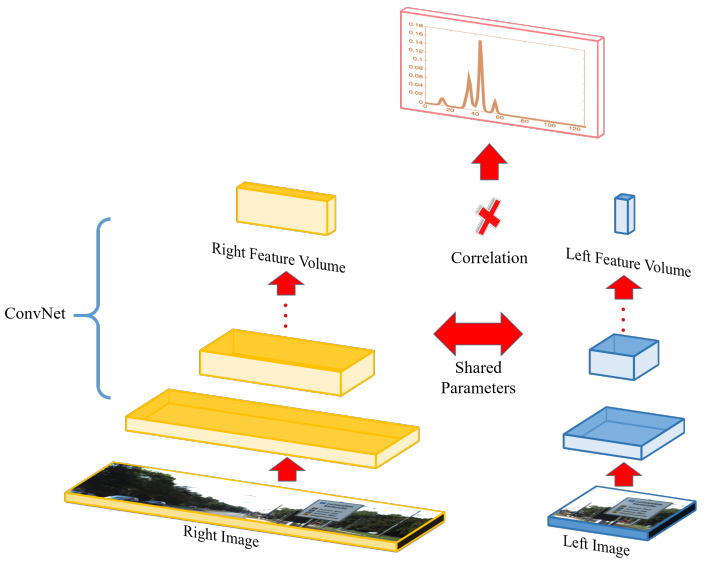
\includegraphics[width=\textwidth]{luo_arch.png}
	\end{subfigure}
	\caption{Αρχιτεκτονικές νευρωνικών δικτύων για την σύγκριση περιοχών εικόνας, όπως προτάθηκαν από τους \e Luo et al. \g \citep{Luo}}
	\label{fig:luo}
\end{figure}

\begin{figure}
	\begin{subfigure}{1\textwidth}
		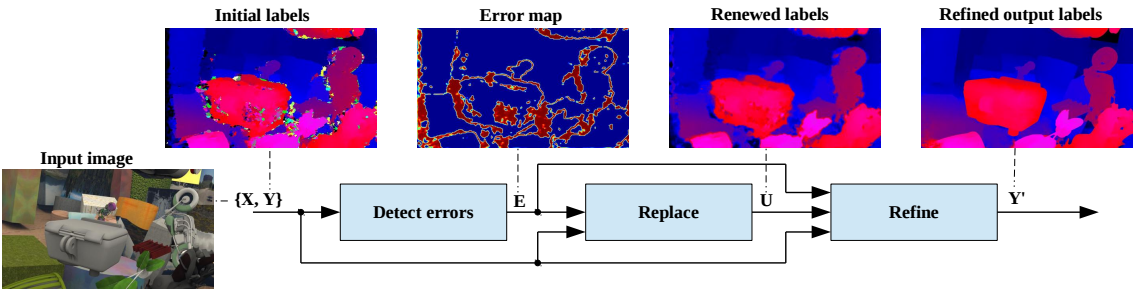
\includegraphics[width=\textwidth]{gidaris_arch.png}
	\end{subfigure}
	\caption{Αρχιτεκτονικές νευρωνικών δικτύων για την σύγκριση περιοχών εικόνας, όπως προτάθηκαν από τους \e Gidaris et al. \g \citep{gidaris2016detect}}
	\label{fig:gydaris}
	\begin{subfigure}{\textwidth}
		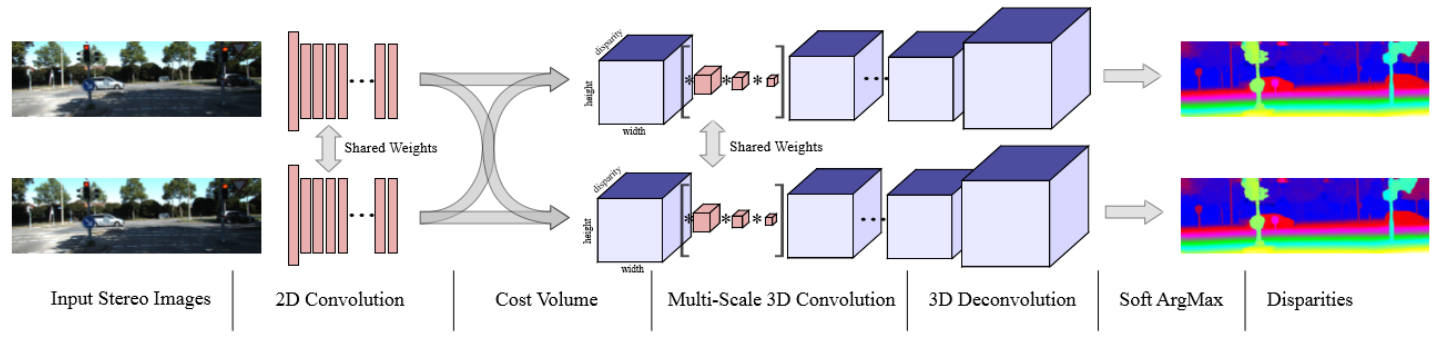
\includegraphics[width=\textwidth]{kendall_arch.png}
	\end{subfigure}
	\caption{Αρχιτεκτονικές νευρωνικών δικτύων για την σύγκριση περιοχών εικόνας, όπως προτάθηκαν από τους \e Kendall et al. \g \citep{gidaris2016detect}}
	\label{fig:kendall}
\end{figure}

	
\section{Επίπεδο κανονικοποίησης δέσμης}
\label{appendix:BN}

	\begin{itemize}
		\item Είσοδος: οι τρισδιάστατοι πίνακες $y_{\mathbf{conv2d}}$ όλης της δέσμης εκπαίδευσης.
		\item 'Εξοδος: οι τρισδιάστατοι πίνακες $y_{\mathbf{BN}}$ όλης της δέσμης εκπαίδευσης, κανονικοποιημένοι με βάση το κάθε ξεχωριστό \e feature map. \g
		\item Διαδικασία: Σε κάθε βήμα εκπαίδευσης, προωθούνται στο δίκτυο $\mathtt{batch\_size}$ εγγραφές του σετ εκπαίδευσης. Κάθε εγγραφή, έχοντας περάσει από το επίπεδο της δισδιάστατης συνέλιξης αναπαρίσταται από έναν πίνακα $y_{conv2d}$. Ο τρισδιάστατος πίνακας $y_{conv2d}$ απαρτίζεται από $\mathtt{f\_maps}$ δισδιάστατους πίνακες $y_{conv2d,i}$. Δημιουργούμε $\mathtt{f\_maps}$ ομάδες, μέλη της οποίας είναι κατ' αντιστοιχία, όλοι οι $\mathtt{batch\_size}$ πίνακες $y_{conv2d,i}$. Τις ομάδες αυτές τις συμβολίζουμε ως $X_j$ και κάθε ξεχωριστό στοιχείου τους ως $X_j^{i}$. Επί αυτών των ομάδων εφαρμόζεται η κανονικοποίηση. Συγκεκριμένα, η κανονικοποίηση δέσμης $X_{\mathbf{BN}, j} = BN_{\gamma, \beta}(X_j) $ υλοποιείται με την ακόλουθη μεθοδολογία:
		
		\begin{equation} \label{eq:batch_normalization}
			\centering
			\begin{split}
				\mu_{X_j} &= \sfrac{1}{m} \sum_{i=1}^{m} X_j^{i} \qquad \qquad \text{// μέσος όρος ομάδας}\\
				\sigma_{X_j}^2 &= \sfrac{1}{m} \sum_{i=1}^{m} (X_j^{i} - \mu_{X_j})^2 \qquad \qquad \text{// διακύμανση ομάδας}\\
				\hat{X_j^{i}} &= \dfrac{X_j^{i} - \mu_{X_j}}{\sqrt{\sigma_{X_j}^2 + \epsilon}} \qquad \qquad \text{// κανονικοποίηση}\\
				\hat{X_j^{i}} &= \gamma \hat{X_j^{i}} + \beta \qquad \qquad \text{// κλιμάκωση και μετατόπιση}
			\end{split}
		\end{equation}
		
Οι μετασχηματισμένες τιμές $\hat{X_j^{i}}$ "αποστοιχίζονται" από τις ομάδες τους κι αναδιατάσσονται στη δομή που είχαν κατά την είσοδό τους στο επίπεδο. Έτσι συνολικά έχει επιτευχθεί η πράξη $y_{\mathbf{BN}} = ΒΝ(y_{\mathbf{conv2d}})$.
	\end{itemize}
	
\section{Συλλογές στερεοσκοπικών δεδομένων με πληροφορία παράλλαξης}
\label{appendix:stereo_dataset}

Οι συλλογές αυτές περιέχουν στερεοσκοπικά ζεύγη μαζί με την πληροφορία παράλλαξης, μετρημένη με κάποιο ειδικό εργαλείο όπως \e lidar \g ή \e laser. \g Η παράλλαξη συνήθως δεν είναι διαθέσιμη στο σύνολο των \e pixels \g του στερεοσκοπικού ζεύγους, αλλά σε ένα υποσύνολο αυτού. Το ποσοστό των διαθέσιμων τιμών επί του συνόλου της εικόνας ονομάζεται πυκνότητα στερεοσκοπικού ζεύγους \e (density of stereo pair): \g

$$\text{πυκνότητα} = \dfrac{\text{διαθέσιμες παραλλάξεις}}{\text{συνολικά \e pixels}}\times 100\%$$

Χαρακτηριστικό μέγεθος κάθε συλλογής είναι η μέση πυκνότητα των εγγραφών της

$$\text{μέση πυκνότητα} = \dfrac{1}{\text{σύνολο στερεοσκοπικών ζευγών}} \sum_{i} \text{πυκνότητα}_i $$

η οποία για προβλήματα πυκνής στερεοσκοπικής αντιστοίχησης \e (dense stereo matching) \g πρέπει να ξεπερνάει το $20\%$.

Οι πιο γνωστές στερεοσκοπικές συλλογές, που θα μας απασχολήσουν στην εργασία, είναι οι \e Middlebury stereo dataset, Kitti stereo benchmark \g και \e Synthetic stereo dataset. \g

\e
\subsection{Middlebury stereo dataset}
\g

Tο σετ δεδομένων \e Middlebury stereo dataset \g δημιουργήθηκε από το ομώνυμο πανεπιστήμιο των Ηνωμένων Πολιτειών το 2001 \cite{scharstein2002taxonomy}. Έκτοτε η συλλογή έχει ανανεωθεί με νέες εκδόσεις τις χρονολογίες 2003 \citep{scharstein2003high}, 2005 \citep{scharstein2007learning}, 2006 \citep{hirschmuller2007evaluation} και 20014 \citep{scharstein2014high}, περιλαμβάνοντας συνολικά περίπου 50 στερεοσκοπικά ζεύγη εικόνων. Οι διάφορες εκδόσεις εμφανίζουν μικρές διαφορές μεταξύ τους καθώς όλες χαρακτηρίζονται από τις παρακάτω ιδιότητες, όπως φαίνεται στην εικόνα \ref{fig:middlebury_example}:

\begin{itemize}
	\item Οι φωτογραφίες έχουν ληφθεί σε εργαστηριακό περιβάλλον ελεγχόμενου φωτισμού
	\item Οι επιφάνειες των αντικειμένων που απαρτίζουν την σκηνή είναι λαμπερτιανές και συνήθως έχουν υφή
	\item οι αυξομειώσεις του βάθους είναι μικρές, άρα και το σύνολο των τιμών παράλλαξης. Προσεγγιστικά $d \in [10,50] \: pixels$
	\item Η πρόσοψη των αντικειμένων εμφανίζει πολύ μικρή κλίση με τον άξονα $zz'$ της στερεοσκοπικής διάταξης 
\end{itemize}

Η μέση πυκνότητα της συλλογής είναι περίπου $97\%$.

Οι δύο εικόνες των στερεοσκοπικών ζευγών έχουν ανάλυση $1988\times2964 \: pixels$, η απόσταση βάσης των δύο λήψεων είναι $B=0.193m$, η εστίαση $f=3997.68 px$ κι η παράλλαξη κυμαίνεται στο διάστημα $[2,265]px$.

\begin{figure}
	\centering
	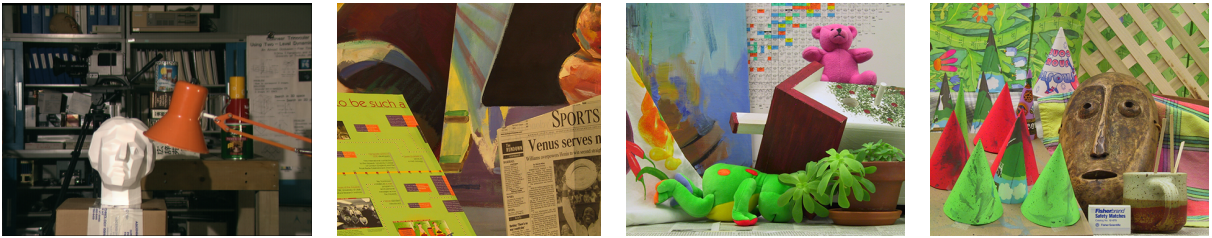
\includegraphics[width=\textwidth]{middlebury_example.png}
	\caption{Παραδείγματα εικόνων από την στερεοσκοπική συλλογή \e middlebury stereo dataset. \g}
	\label{fig:middlebury_example}
\end{figure}

\e
\subsection{Kitti stereo benchmark}
\g

Η συλλογή δεδομένων \e Kitti stereo benchmark \g δημιουργήθηκε το 2012 \cite{geiger2012we} από το τεχνολογικό Ινστιτούτο της Καρλσρούης \e (Karlsruhe institute of Technology) \g σε συνεργασία με το τεχνολογικό Ινστιτούτο της Τογιότα στο Σικάγο \e (Toyota Technological Institute at Chicago). \g Ανανεώθηκε το 2015 \citep{menze2015object} περιλαμβάνοντας πλέον συνολικά 400 στερεοσκοπικά ζεύγη εικόνων.

Οι εικόνες έχουν ληφθεί από την οροφή ενός αυτοκινήτου \ref{fig:kitti_car}. Το πραγματικό βάθος των απεικονιζόμενων αντικειμένων έχει ληφθεί από στρεφόμενο σαρωτή λέιζερ \e (rotating laser scanner) \g τοποθετημένο πίσω από την αριστερή κάμερα.

Η γεωμετρία και στατιστική των εικόνων που περιλαμβάνει διαφέρει πλήρως από αυτή του \e Middlebury stereo dataset \g καθώς χαρακτηρίζεται από τις εξής ιδιότητες:

\begin{itemize}
	\item Οι φωτογραφίες έχουν ληφθεί σε φυσικό περιβάλλον, στους δρόμους της Καρλσρούης μια ηλιόλουστη ημέρα. Περιλαμβάνουν κατά κύριο λόγο κινούμενα οχήματα, πεζοδρόμια, πεζούς και σπίτια εκατέρωθεν του δρόμου.
	\item Οι επιφάνειες των αντικειμένων που απαρτίζουν την σκηνή είναι δεν είναι στο σύνολό τους λαμπερτιανές. Ταυτόχρονα ο έντονος ήλιος δρα ως μια πολύ δυνατή πηγή φωτός με αποτέλεσμα να δημιουργούνται έντονα φαινόμενα κατοπτρικών ανακλάσεων.\footnote{Στην ανανέωση του 2015 τα τζάμια των αυτοκινήτων περιέχουν πληροφορία παράλλαξης και συμπεριλαμβάνονται στην αξιολόγηση, κάνοντας τη συλλογή πιο απαιτητική στον χειρισμό των κατοπτρικών επιφανειών}
	\item Η έντονη πηγή φωτός δημιουργεί συχνά κορεσμό στον αισθητήρα $ccd$ με αποτέλεσμα την αποτύπωση ειδώλων χωρίς υφή.
	\item οι αυξομειώσεις του βάθους, άρα και το σύνολο των τιμών παράλλαξης, είναι πολύ μεγάλο.
	\item Οι προσόψεις των αντικειμένων εμφανίζουν μεγάλες κλίση, σε σχέση με τον άξονα $zz'$ της στερεοσκοπικής διάταξης δημιουργώντας εντονότερα φαινόμενα αυξομείωσης αποστάσεων και αποκρύψεων.
\end{itemize}

Η μέση πυκνότητα της συλλογής είναι περίπου $20\%$.

Οι δύο εικόνες των στερεοσκοπικών ζευγών έχουν ανάλυση $376\times1241 \: pixels$, η απόσταση βάσης των δύο λήψεων είναι $B=0.54m$, η εστίαση $f=707.09 px$ κι η παράλλαξη κυμαίνεται στο διάστημα $[0,230]px$.

Στην εικόνα \ref{fig:midd_kitti_differences} αποτυπώνονται παραστατικά οι έντονες διαφορές ανάμεσα στις συλλογές \e KITTI \g και \e Middlebury. \g

\begin{figure}
	\centering
	\begin{subfigure}{0.49\textwidth}
		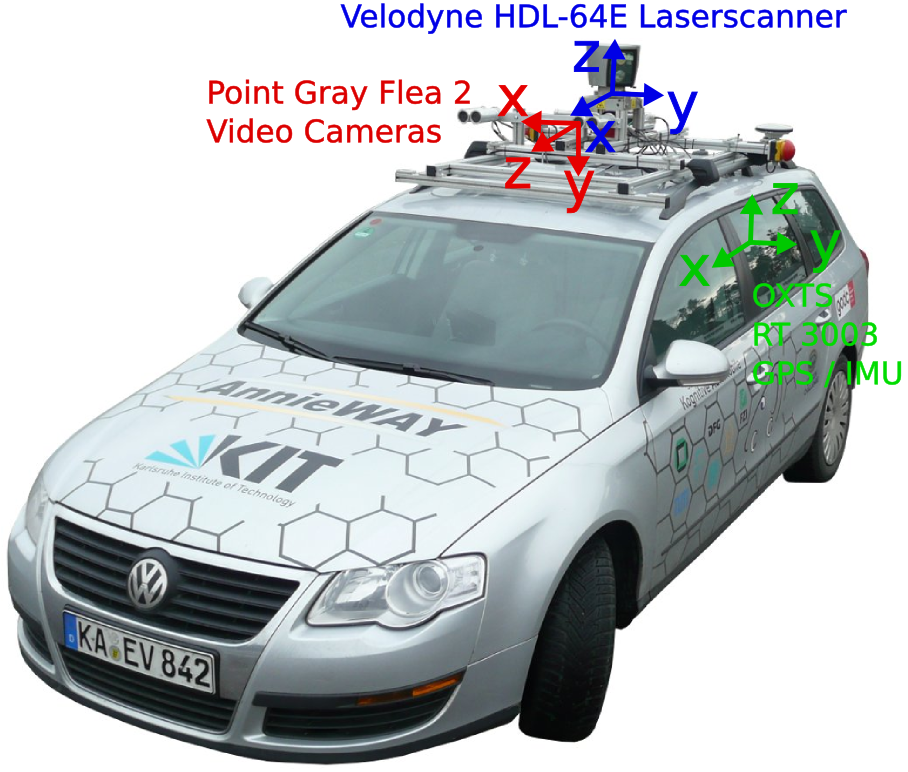
\includegraphics[width=\textwidth]{kitti_car.png}
	\end{subfigure}
	\begin{subfigure}{0.49\textwidth}
		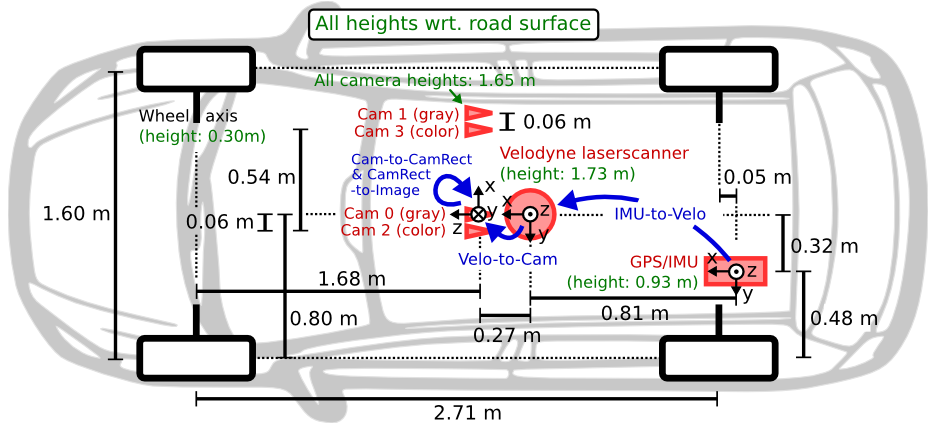
\includegraphics[width=\textwidth]{kitti_car_profile.png}
	\end{subfigure}
	\caption{Το αυτοκίνητο που χρησιμοποιήθηκε για την συλλογή \e KITTI \g και η κάτοψή του.}
	\label{fig:kitti_car}
\end{figure}

\begin{figure}
	\centering
	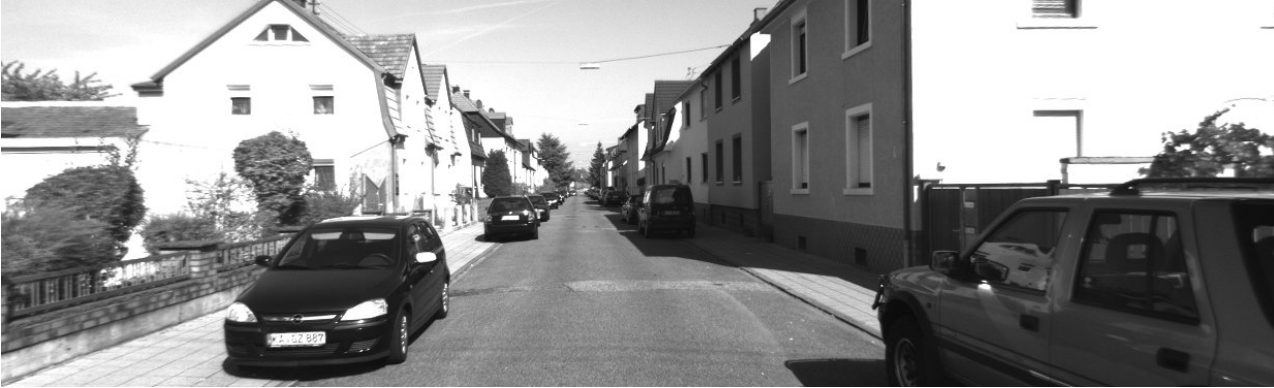
\includegraphics[width=\textwidth]{kitti_example.png}
	\caption{Παραδείγμα εικόνας από την στερεοσκοπική συλλογή \e kitti stereo benchmark. \g}
	\label{fig:kitti_example}
\end{figure}

\begin{figure}
	\centering
	\begin{subfigure}{\textwidth}
		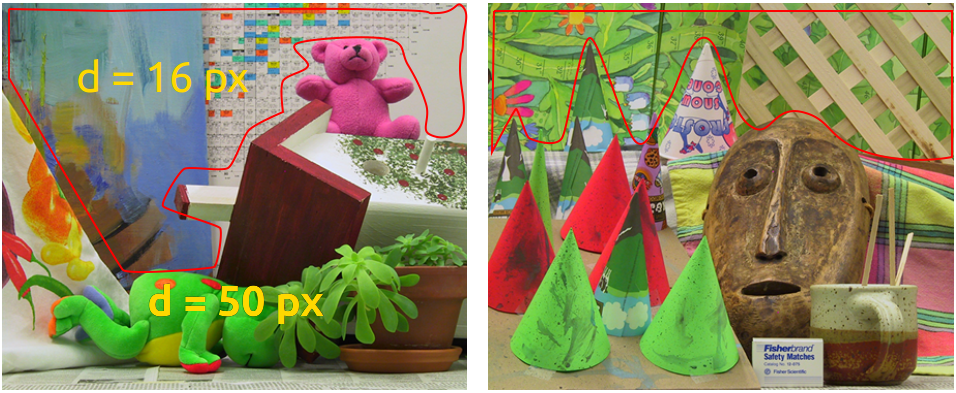
\includegraphics[width=\textwidth]{middlebury_example_1.png}
	\end{subfigure}
	\begin{subfigure}{\textwidth}
		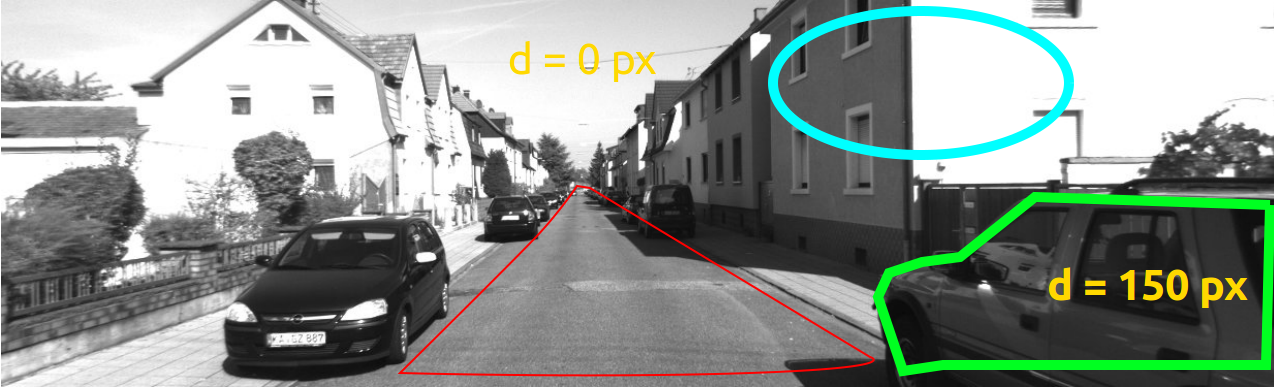
\includegraphics[width=\textwidth]{kitti_example_1.png}
	\end{subfigure}
	\caption{\textbf{Κίτρινα χρώμα:} μέγιστη κι ελάχιστη τιμή παράλλαξης σε κάθε εικόνα. \textbf{Κόκκινο χωρίο:} διαφορά στην κλίση των εικονιζόμενων αντικειμένων. \textbf{Πράσινο χωρίο:} παράδειγμα κατοπτρικής ανάκλασης. \textbf{Γαλάζιο χωρίο:} παράδειγμα κορεσμού αισθητήρα λόγω έντονου φωτός, με αποτέλεσμα την απεικόνιση επιφάνειας χωρίς υφή}
	\label{fig:midd_kitti_differences}
\end{figure}


\e
\subsection{Synthetic stereo dataset}
\g
Το 2015, οι \e Mayer et al. \cite{mayer2016large} \g δημιούργησαν μια μεγάλη συνθετική συλλογή από στερεοσκοπικά ζεύγη. Η συλλογή αυτή προσεγγίζει σε ομοιότητα φυσικές εικόνες και ταυτόχρονα περιέχει πάρα πολλά στερεοσκοπικά ζεύγη (35.000) αποτελώντας βάση δεδομένων για την εκπαίδευση αλγορίθμων εκμάθησης μηχανής. Στην παρούσα εργασία δεν αξιοποιούμε την υπάρχουσα συλλογή. Παραδείγματα εικόνων της στερεοσκοπικής συλλογής φαίνονται στο σχήμα \ref{fig:synthetic_dataset}.

\begin{figure}
	\centering
	\begin{subfigure}{0.6\textwidth}
		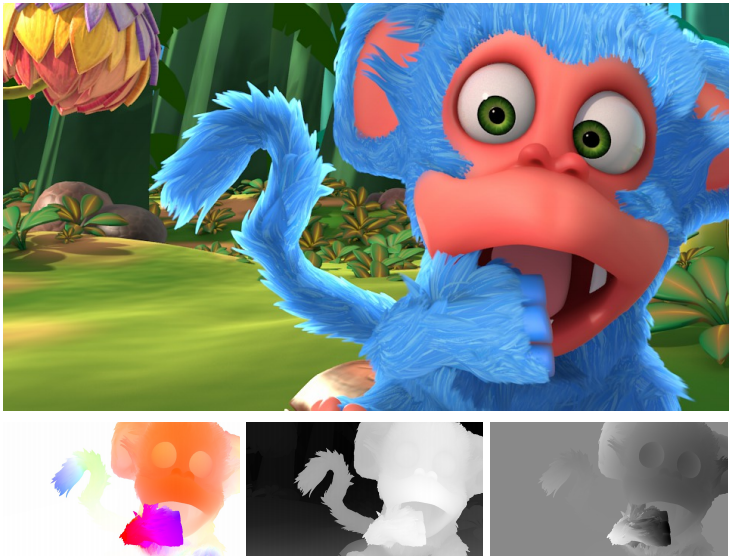
\includegraphics[width=\textwidth]{synthetic_dataset.png}
		\caption{Εικόνα από την συνθετική συλλογή}
	\end{subfigure}
	\begin{subfigure}{\textwidth}
		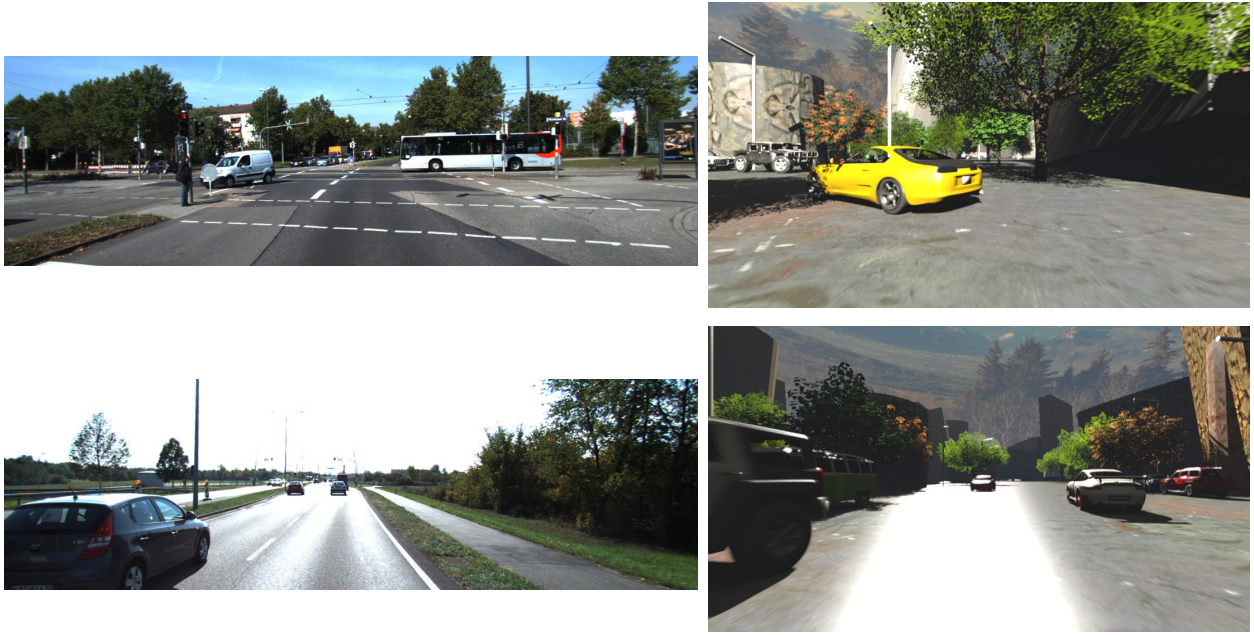
\includegraphics[width=\textwidth]{synthetic_kitti_dataset.png}
		\caption{Σύγκριση εικόνων δρόμου συνθετικής συλλογής (δεξιά) και συλλογής \e kitti stereo benchmark \g (αριστερά)}
	\end{subfigure}
	\caption{Συνθετική συλλογή στερεοσκοπικών εικόνων}
	\label{fig:synthetic_dataset}
\end{figure}


\section{Αναλυτική περιγραφή της δημιουργίας του σετ εκπαίδευσης}
\label{appendix:dataset_creation}

Οι εγγραφές δημιουργούνται με την ακόλουθη μεθοδολογία. Ως εικόνα αναφοράς θεωρούμε την αριστερή εικόνα του στερεοσκοπικού ζεύγους. Σε κάθε σημείο \e $\textbf{p} = (x,y) \in I^L$ \g όπου ισχύουν οι τρεις παρακάτω προϋποθέσεις:
\begin{itemize}
	\item η τιμή της παράλλαξης είναι γνωστή
	\item \e $\texttt{max\_disparity} + \dfrac{n-1}{2} < x < \text{width} - \dfrac{n-1}{2}$ \g, 
	\item \e $\dfrac{n-1}{2} < y < \text{height} - \dfrac{n-1}{2}$ \g
\end{itemize}

εφαρμόζουμε την εξής μεθοδολογία:

\begin{itemize}
	\item Αποθηκεύουμε το τετράγωνο χωρίο διαστάσεων $n \times n$ \e pixels \g πέριξ του σημείου \e $\textbf{p}$ \g ως \e $\mathcal{P}_{n \times n}^L(\mathbf{p})$. \g 
	\item Αποθηκεύουμε το παραλληλόγραμμο χωρίο διαστάσεων \e $( \texttt{max\_disparity} + n) \times n$ \g ως \e $\mathcal{P}_{( \texttt{max\_disparity} + n) \times n}^R(\mathbf{q})$ \g. Η θέση \e $\mathbf{q}$ \g υπολογίζεται ως 
	\e $$\mathbf{q} = \texttt{int}(x - d, y)$$ \g και το χωρίο εκτείνεται:
	\begin{itemize}
		\item $\dfrac{n-1}{2}$ θέσεις προς τα πάνω, κάτω και δεξιά
		\item \e $\texttt{max\_disparity} + \dfrac{n-1}{2}$ \g θέσεις προς τα αριστερά
	\end{itemize}
	\item Αναθέτουμε ως \e label \g την τιμή της παράλλαξης του σημείου. Η ετικέτα \e label \g λαμβάνει τιμές στο διάστημα \e $[0,\texttt{max\_disparity}]$ \g
\end{itemize}

Ουσιαστικά κάθε εγγραφή εκπαίδευση περιέχει το χωρίο αναφοράς $\mathcal{P}_{n \times n}^L(\mathbf{p})$ και όλα τα πιθανά χωρία που αυτό θα μπορούσε να αποτυπώνεται στην έτερη λήψη \e $\mathcal{P}_{( \texttt{max\_disparity} + n) \times n}^R(\mathbf{q})$. \g

\section{Επεξήγηση σχέσης \ref{eq:total_minima}}
\label{appendix:minimum_explanation}

Ο λόγος που μας ενδιαφέρει η προσέγγιση της ελάχιστης τιμής, κι όχι η εύρεσή της, είναι ότι οι παράμετροι που οδηγούν στην ελάχιστη τιμή αυτή καθ' αυτή, είναι ευάλωτοι σε υπερπροσαρμογή \e (overfitting). \g Το ολικό ελάχιστο της συνάρτησης είναι έντονα επηρεασμένο από την τυχαία μορφή των συγκεκριμένων παραδειγμάτων $X$, ενώ η ευρύτερη περιοχή πέριξ αυτού αναπαριστά καλύτερα το γενικό μοτίβο που ακολουθούν τα παραδείγματα εκπαίδευσης και που τελικά θέλουμε το δίκτυό μας να "μάθει". Ο παραπάνω σχολιασμός θα είχε μεγαλύτερη αξία εάν εκπαιδεύαμε το δίκτυο πάνω σε \textbf{όλα} τα δεδομένα του σετ εκπαίδευσης μέσω του αλγορίθμου "απότομης καθόδου" \e (gradient descent). \g Η επιλογή μας να χρησιμοποιήσουμε την εναλλακτική μορφή του αλγορίθμου "στοχαστικής απότομης καθόδου μικρής δέσμης" \e (mini-batch stochastic gradient descent) \g μας απαλλάσσει από τον παραπάνω προβληματισμό, καθώς το δίκτυο αναπροσαρμόζει τις παραμέτρους του επιλύοντας διαρκώς διαφορετικά προβλήματα ελαχίστου, το καθένα βασισμένο σε ένα διαφορετικό υποσύνολο παραδειγμάτων της συλλογής εκπαίδευσης. Επομένως, είναι σχεδόν βέβαιο ότι με μια μικρή αναπροσαρμογή παραμέτρων στην κατεύθυνση του εκάστοτε ελαχίστου, το δίκτυο δεν θα φτάσει ποτέ ούτως ή άλλως στο ολικό ελάχιστο, παρά μόνο θα το προσεγγίζει, ικανοποιώντας την συνθήκη \ref{eq:total_minima}.

\section{Περιγραφή μεθόδων τις οποίες συνδυάζει ο αλγόριθμος \texorpdfstring{\e ADAM \g}{TEXT}}
\label{appendix:adam_explanation}

Σε κάθε βήμα, οι παράμετροι $W$ ανανεώνονται ως:

$$W_{i+1} = W_i - \mathtt{learning\_rate} \times \bigtriangledown_{W_i}f(X_i,W_i)$$

Αυτή η απλή εκδοχή του αλγορίθμου "στοχαστικής απότομης καθόδου μικρής δέσμης" \e (mini-batch stochastic gradient descent) \g δυσκολεύευται σε περιοχές που η κλίση αποκλίνει από διάσταση σε διάσταση, δηλαδή το διάνυσμα $\bigtriangledown_{W_i}f(X_i,W_i)$ εμφανίζει μεγάλη διακύμανση. Τέτοια "φυσιολογία" συνηθίζουν να εμφανίζουν οι περιοχές κοντά στα τοπικά ελάχιστα, όπου ο αλγόριθμος "ταλαντώνεται" ανάμεσα στις δύο "πλαγιές" πλησιάζοντας πολύ διστακτικά το τοπικό ελάχιστο. Για τον λόγο αυτό εισάγεται στην ανανέωση των παραμέτρων ο όρος momentum $v$. Μπορούμε να παρομοιάσουμε αυτή την εκδοχή του αλγορίθμου με μία μπάλα που αφήνουμε να κατρακυλήσει στην πλαγιά ενός λόφου. Η πορεία που ακολουθεί δεν εξαρτάται μόνο από την κλίση του εδάφους σε κάθε σημείο, αλλά και από την ταχύτητα που έχει ήδη αναπτύξει. Έτσι πραγματοποιείται ταχύτερη σύγκλιση στο τοπικό ελάχιστο. Η συνηθισμένη τιμή της παραμέτρου $\mathtt{momentum\_rate}$ κινείται κοντά στο $0.9$.

$$v_{i+1} = \mathtt{momentum\_rate} \times v_{i} + \mathtt{learning\_rate} \times \bigtriangledown_{W_i}f(X_i,W_i)$$
$$W_{i+1} =W_{i} - v_{i+1}$$

Οι παραπάνω μέθοδοι αναπροσαρμόζουν τις τιμές των παραμέτρων κατά σταθερό $\mathtt{learning\_rate}$. Η εύρεση της κατάλληλης τιμής $\mathtt{learning\_rate}$ απαιτεί χρονοβόρο πειραματισμό. Προς επίλυση αυτής της προβληματικής, έχουν αναπτυχθεί αλγόριθμοι που αυξομειώνουν εσωτερικά το $\mathtt{learning\_rate}$. Πιο συγκεκριμένα, ο αλγόριθμος \e RMSprop \g δημιουργεί έναν κινούμενο μέσο όρο που ρυθμίζει το $\mathtt{learning\_rate}$ διαφορετικά για κάθε διάσταση σύμφωνα με τον ακόλουθο κανόνα:
Συμβολίζουμε ως $\mathbf{record}$ το διάνυσμα ίδιων διαστάσεων με το διάνυσμα παραμέτρων $W$ που κρατάει το "ιστορικό" των μεταβολών:

\begin{equation}
	\begin{split}
		\mathbf{record} &= \mathtt{decay\_rate} \cdot \mathbf{record}+ (1-\mathtt{decay\_rate}) \nabla_{W_{i}}f^2(X_i,W_i)
	\end{split}
\end{equation}

$$W_{i+1} = \dfrac{-\mathtt{learning\_rate} \cdot \nabla_{W_{i}}f(X_i,W_i)}{\sqrt{\mathbf{record} + \epsilon}}$$
	

